\documentclass[12pt]{article}

\RequirePackage{lineno}
\setlength{\linenumbersep}{6pt}
%\linenumbers

\usepackage{graphicx}
\usepackage{subfigure}
\usepackage{dcolumn}
\usepackage{comment}
\usepackage{bm}
\usepackage{amssymb}
\usepackage{multirow}

%%%%%%%%%%%%%%%%%%%%
\usepackage{hyperref} %using hypertext
%%%%%%%%%%%%%%%%%%%%

\setlength{\textwidth}{17.5cm}
\setlength{\textheight}{24cm}
\setlength{\oddsidemargin}{-.3cm}
\setlength{\evensidemargin}{-.3cm}
\setlength{\topmargin}{-2.0cm} %%%for mjt
%\setlength{\topmargin}{0.0cm}  %%%for Jan



\def\defn#1{{\color{red} #1}}
\def\tred#1{{\color{red} #1}}
\def\tblue#1{{\color{blue} #1}}

\def\fig#1{Fig.~\ref{#1}}
\def\eq#1{Eq.~(\ref{#1})}
\def\tab#1{Tab.~\ref{#1}}

%bold in math mode
\def\mbold#1{\mbox{\boldmath\ensuremath{#1}}} 
%definition symbol. When you type just := the : sum is vertically misaligned
\def\defeq{\mathrel{\mathop:}=}

\def\acosh{\mbox{\rm acosh}}
\def\asinh{\mbox{\rm asinh}}

\def\gev{\mbox{~GeV}}
\def\gevc{\mbox{~GeV/$c$}}
\def\gevcc{\mbox{~GeV/$c^2$}}
\def\mevc{\mbox{~MeV/$c$}}

\def\la{\left<}
\def\ra{\right>}

\def\mean#1{\ensuremath{\la#1\ra}}
\def\meanabs#1{\ensuremath{\la|#1|\ra}}
\def\meankv#1{\ensuremath{\la#1^2\ra}}
\def\rms#1{\meankv{#1}}
\def\sqrtrms#1{\ensuremath{\sqrt{\meankv{#1}}}}

\def\eg{{\it e.g.}}
\def\etc{{\it etc}}
\def\etall{{\it et al.}}

\def\ptq#1{\ensuremath{\hat{p}_{\rm T#1}}} 
\def\ptqkv#1{\ensuremath{\hat{p}^2_{\rm T#1}}} 
\def\vptq#1{\ensuremath{\vec{\hat{p}}_{\rm T#1}}} 
\def\ptg{\ensuremath{p_{\rm T\gamma}}} 

\def\pt#1{\ensuremath{p_{\rm T#1}}} 
\def\ptkv#1{\ensuremath{p^2_{\rm T#1}}} 
\def\vpt#1{\ensuremath{\vec{p}_{\rm T#1}}} 
\def\et{\ensuremath{E_{\rm T}}} 

\def\kt#1{\ensuremath{k_{\rm T#1}}} 
\def\ktkv#1{\ensuremath{k^2_{\rm T#1}}} 
\def\vkt#1{\ensuremath{\vec{k}_{\rm T#1}}} 

\def\jt#1{\ensuremath{j_{\rm T#1}}} 
\def\jtkv#1{\ensuremath{j^2_{\rm T#1}}} 
\def\vjt#1{\ensuremath{\vec{j}_{\rm T#1}}} 

\def\mkv#1{\ensuremath{m^2_{#1}}}
\def\mt#1{\ensuremath{m_{\rm T#1}}}
\def\mtkv#1{\ensuremath{m^2_{\rm T#1}}}

\newcommand{\sign} {\ensuremath{\sigma_{\rm N}}}
\newcommand{\siga} {\ensuremath{\sigma_{\rm A}}}
\newcommand{\yn} {\ensuremath{Y_{\rm N}}}
\newcommand{\yf} {\ensuremath{Y_{\rm F}}}
%\newcommand{\D} {\ensuremath{D^q_\pi}}
\newcommand{\D} {\ensuremath{D^f}}
\newcommand{\fq}{\ensuremath{f_Q(\hat{p}_T)}}
\newcommand{\sq}{\ensuremath{\Sigma_Q(\hat{p}_T)}}
\newcommand{\fkt}{\ensuremath{f^\prime_Q(\hat{p}_{\rm Tt})}}
\newcommand{\skt}{\ensuremath{\Sigma^\prime_Q(\hat{p}_{\rm Tt})}}
\newcommand{\prob}{\ensuremath{\mathcal{P}}}

%\newcommand{\condta}{\ensuremath{\Big|_{\pt{t},\pt{a}}}}
% \left.something \right|_{xy}

\newcommand{\auau} {\ensuremath{Au+Au}}
\newcommand{\hi} {\ensuremath{A+A}}
\newcommand{\dau} {\ensuremath{d+Au}}
\newcommand{\pp} {\ensuremath{p+p}}
\newcommand{\ee} {\ensuremath{e^+ + e^-}}

\newcommand{\mpt} {\mean{\pt{}}} 
\newcommand{\ptt}{\ensuremath{p_{\rm Tt}}}
\newcommand{\mptt} {\mean{\ptt}} 
\newcommand{\pta}{\ensuremath{p_{\rm Ta}}}
\newcommand{\mpta} {\mean{\pta}} 
\def\pn{\ensuremath{\hat{p}_{\rm n}}} 
\def\pnkv{\ensuremath{\hat{p}^2_{\rm n}}} 
\def\vpn{\ensuremath{\vec{\hat{p}}_{\rm n}}} 

\newcommand{\pout} {\ensuremath{p_{\rm out}}}
\newcommand{\qout} {\ensuremath{\hat{p}_{\rm out}}}

\newcommand{\mz} {\mean{z}}
\newcommand{\zt} {\ensuremath{z_{\rm t}}}
\newcommand{\mzt} {\mean{\zt}}
\newcommand{\za} {\ensuremath{z_{\rm a}}}
\newcommand{\mza} {\mean{\za}}
\newcommand{\xe} {\ensuremath{x_{\rm E}}}
\newcommand{\xh} {\ensuremath{x_{\rm h}}}
\newcommand{\xhq} {\ensuremath{\hat{x}_{\rm h}}}
\newcommand{\zkt} {\ensuremath{ \mean{\zt}\sqrtrms{\kt{}} }}
\newcommand{\xzkt} {\ensuremath{ \xhq^{-1}\mean{\zt}\sqrtrms{\kt{}} }}
\newcommand{\xzktfull} {\ensuremath{ \xhq^{-1}(\kt{},\xh)\mean{\zt(\kt{},\xh)}\sqrtrms{\kt{}} }}

\newcommand{\snn} {\ensuremath{\sqrt{s_{\rm NN}}}}
\newcommand{\s} {\ensuremath{\sqrt{s}}}
\newcommand{\piz} {\ensuremath{\pi^0}}
\newcommand{\pizh}{\ensuremath{\pi^0-h^\pm}}
\newcommand{\gammah}{\ensuremath{\rm direct-\gamma-h^\pm}}
\newcommand{\pipmh}{\ensuremath{\pi^\pm-h^\pm}}
\newcommand{\hh}{\ensuremath{h^\pm-h^\pm}}

\newcommand{\pbar} {\ensuremath{\overline{p}}}
\newcommand{\lbar} {\ensuremath{\overline{\Lambda}}}
\newcommand{\npart} {\ensuremath{N_{\rm part}}}
\newcommand{\npartav} {\ensuremath{\la N_{\rm part} \ra}}
\newcommand{\ncoll} {\ensuremath{N_{\rm coll}}}
\newcommand{\ncollav} {\ensuremath{\la N_{\rm coll} \ra}}
\newcommand{\ut} {\ensuremath{\la u_t \ra}}

\newcommand{\alphas} {\ensuremath{\alpha_{s}}}
\newcommand{\alphasQ} {\ensuremath{\alpha_{s}(Q^2)}}
\newcommand{\dphi} {\ensuremath{\Delta \phi}}
\newcommand{\xt} {\ensuremath{x_{\rm T}}}
\newcommand{\xtt} {\ensuremath{x_{\rm Tt}}}
\newcommand{\rmskt} {\ensuremath{ \sqrt{\mean{{\kt{}^2}} }}}

\newcommand{\spn} {\ensuremath{\sigma}}
\newcommand{\ptaf} {\ensuremath{\mathbf{\ptq{a}}}}
\newcommand{\pttf} {\ensuremath{\mathbf{\ptq{t}}}}

%%%MJT Added 012611
\def\lsim{\raise0.3ex\hbox{$<$\kern-0.75em\raise-1.1ex\hbox{$\sim$}}}
\def\gsim{\raise0.3ex\hbox{$>$\kern-0.75em\raise-1.1ex\hbox{$\sim$}}}


\begin{document}

\title{Parent Child Relationship}
\author{Jan Rak}
\date{}
\maketitle

%------------------------------------------------------------------------------------------------------
\section{``Parent-child relationship'' and the trigger bias} \label{sec:parent-child}

As originally indicated by Bjorken in \cite{Bjorken:1973kd}  (see also \cite{Adler:2006sc} and \cite{Tannenbaum:2006ku}) the particle 
\pt{} distribution has the same, or very similar, shape as  the jet cross section. This is known as a ``Parent-Child Relationship'' (PCR) and  follows from the observations: 
\begin{itemize}
\item At sufficiently high transverse momentum (\pt{}$\gtrsim$3 \gevc) the inclusive \pt{}-distribution can be quite accurately approximated by a power law function. It reflects the nature of the lowest order 2$\rightarrow$2 hard scattering dominated by a  single vector boson exchange (gluon). It can be shown that in this case the \pt{}-distribution of the final state jets follows the $\pt{}^{-4}$ power law distribution \cite{Feynman1}. In reality, the jet \pt{} spectrum is steeper due to the effect of soft QCD radiation, and scaling violation, but the power law shape is retained. Authors of \cite{Jacob:1978mj} argued that this relation holds for power law  with a constant power. However, strictly speaking, PCR holds for parton spectrum shape which can be characterized by any function having a property $f(x\cdot y)=f(x)\cdot f(y)$. 
\item Fragmentation function, $\D(z)$ is a universal function of the momentum fraction $z=\pt{}/\ptq{}$ where $\pt{}$ and $\ptq{}$ are the transverse momenta of the fragment and jet respectively. FF is independent of the parton momentum and thus universal. This is obviously only an approximation. In reality the fragmentation function depends on parton momentum as well (scaling violation). However, it is save to assume that these effects are not relevant for the analysis presented here. Here we also ignore the partons flavor. 
\end{itemize}


%The final particle \pt{}-distribution can be evaluated as a folding of the jet spectrum with the fragmentation function. 
%If the scaling violation can be neglected then this folding does not change the the shape (see \eq{eq:foldingJetSpect}) 
%\begin{equation}\label{eq:foldingJetSpect}
%\frac{d\sigma}{dpt{}}=\int_{\ptq{}>\pt{}}d\ptq{}\frac{d\sigma^{\rm jet}}{d\ptq{}}\int_{0}^{1}dz\D(z)\delta(\pt{}-z\ptq{})
%\end{equation}

The joint probability of detecting a hadron with \pt{}$=z\ptq{}$  originating from a parton of \ptq{}\ can be written as
\begin{equation} \label{eq:jointprob}
{d^2P_{q\rightarrow h}\over d\ptq{}dz}  =  {dP_q \over d\ptq{}}\times\D(z)
\end{equation}
where the parton spectrum $ {dP_q / d\ptq{}} =  \hat{C}\ptq{}^{1-n}$ and $\D(z)$ is the fragmentation function. Power law exponent $1-n$ is 
chosen such that $n$ represents the exponent of the invariant cross section 
\begin{equation}\label{eq:powerlawf}
{d\sigma_q\over\ptq{}d\ptq{}}  \equiv f_q(\ptq{}) = \hat{C}\ptq{}^{-n}\ .
\end{equation}
With a simple change of variables from \ptq{}\ to \pt{}$=z\ptq{}$, one obtains the joint probability 
\begin{equation} \label{eq:jointprobInv}
{d^2\sigma_h\over d\ptq{}dz}  = 
        {d^2\sigma_h\over z^{-1}d\pt{}dz} 
    %\makebox[5 mm]{}\rightarrow \makebox[5 mm]{}
    \rightarrow
        {d^2\sigma_h\over d\pt{}dz} = \hat{C}\left({p_T\over z}\right)^{1-n}\cdot\D(z)\cdot{1\over z}
    %\makebox[5 mm]{}\rightarrow \makebox[5 mm]{}
    \rightarrow
         {d^2\sigma_h\over\pt{}d\pt{}dz} = f_q(\ptq{})\cdot\D(z)\cdot{1\over z^2}\ \cdot
\end{equation}
The \pt{}\ and $z$ dependencies do not factorize. However, the \pt{}\ spectrum may be
found by integrating over all values of \ptq{}\ $\geq$ \pt{}\ to \ptq{}$_{max}=\sqrt{s}/2$,
which corresponds to values of $z$ from $x_T=2 p_T/\sqrt{s}$ to 1.
\begin{equation}
\label{eq:dsigma_integral}
{1\over \pt{}}{d\sigma_h\over d\pt{}}  =
    \int_{\xt}^{1} \hat{C}\left({\pt{}\over z}\right)^{-n}\D(z)\; {dz\over z^{2}}=
    \hat{C}\pt{}^{-n}\int_{\xt}^{1} \D(z) z^{n-2}dz \ \propto\ C\pt{}^{-n}
\end{equation}
Last integral in \eq{eq:dsigma_integral} depends only weakly on \pt{} due to the lower boundary \xt{} (actually at \s=7 TeV there is no dependence up to $\sim$ 500 \gevc) and thus the \eq{eq:dsigma_integral} demonstrates that up to a constant factor the partonic and hadronic invariant cross sections are identical.

The second important feature of \eq{eq:dsigma_integral} is the factor $z^{n-2}$ under the integral. It implies that the inclusive particle 
takes the large momentum fraction from the trigger jet. This is know as a ``trigger bias''. 

\subsection{Moment of the Fragmentation Function}

Here I denote the first moment of some quantity $x$ over the distribution $f(x)$  as $\mean{x}$. Since many of the functions
discussed below are not normalized to the unity then:
\begin{equation}
\mean{x^{n}} = E[x^n]/E[x^0]\equiv \int x^{n}f(x)dx
\end{equation}
where $E[x^{n}]$ denotes an expectation value. I will thus ignore the normalization.

When the fragmentation function is approximated by an exponential function $\D(z)=\exp(-\alpha z)$, where $\alpha=8.4$ for quark and $\alpha=11.3$ \cite{Adler:2006sc} then  by use of incomplete Gamma function
\footnote{ $\Gamma(s,x)=\int_{x}^{\infty} e^{-t}t^{s-1}dt$ }, 
\eq{eq:powerlawf} and assumption $\xt\to1$:
\begin{eqnarray}
\label{eq:meanz_inc}
\mean{ z_{\rm inc}} 	&=&   {\int_{\xt}^{1}\D(z)\;   {dP_q \over d\ptq{}} \;      {dz\over z^{2}}} 
				  =   \int_{\xt}^{1} dz \cdot\D(z)\cdot z^{n-3}  \\ \nonumber
				&\approx& \int_{0}^{1}dz\; e^{-\alpha z}\cdot z^{n-3} = 
				{1\over \alpha}\cdot{\Gamma(n-1)-\Gamma(n-1,\alpha) \over \Gamma(n-2)-\Gamma(n-2,\alpha) }
\end{eqnarray}

%When we ignore the lower integration limit ($\xt~0$) then the $\mean{ z_{\rm inc}(\pt{}) }$ can be evaluated using a moment generating function:
%\begin{equation}
%\mean{ z_{\rm inc}(\pt{}) } = \left. {d\over dt} \int_{\xt}^{1} dz \cdot e^{t.z}\D(z)\cdot z^{n-2} \right|_{t=0}
%\end{equation}

Using \eq{eq:meanz_inc} one can calculate the mean momentum fraction of inclusive particle production as a function of the power law exponent $n$ (\eq{eq:powerlawf}). See \fig{fig:meanz}. The slopes of exponential $\D(z)$ are taken from \cite{Adler:2006sc} and the vertical lines indicates measured power law exponent of $h^{\pm}$ production measured at RHIC \cite{Adler:2006bw} $n_{\rm 0.2 TeV}=8.10\pm 0.05$ and LHC pp \s=0.9 TeV $n_{\rm 0.9 TeV}=6.63\pm0.12$ \cite{Aamodt:2010my}

\begin{figure}[htbp]
\centering
\resizebox{0.49\columnwidth}{!}{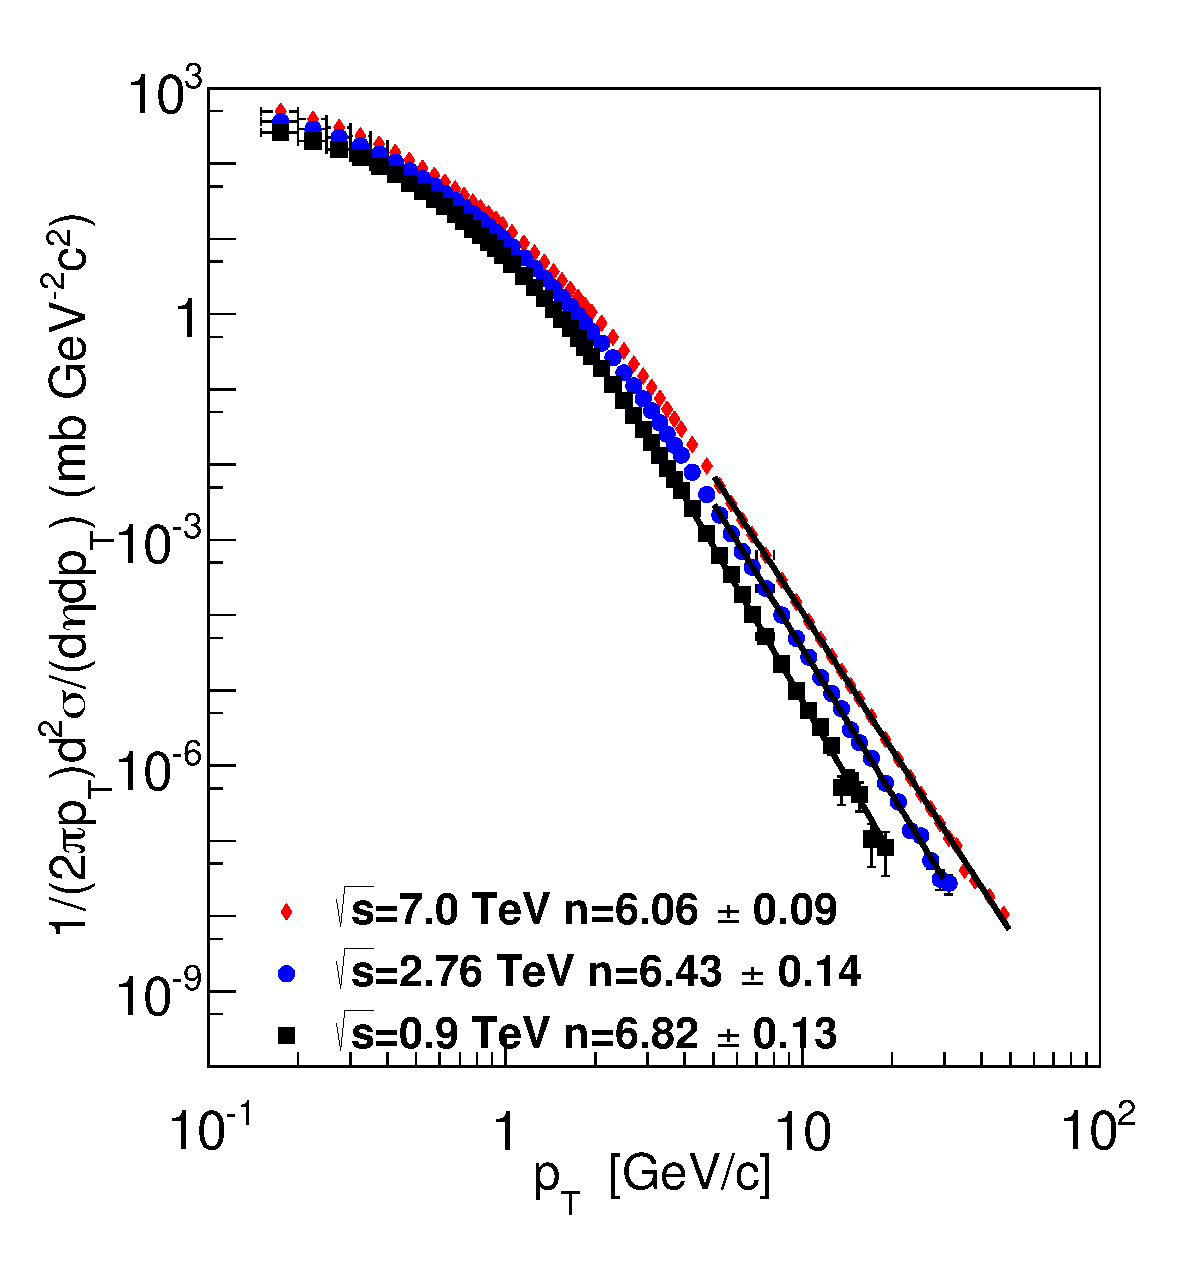
\includegraphics{figs/ALICE_pp}}
\resizebox{0.49\columnwidth}{!}{\includegraphics{math/gamma}}
\caption{ }
\label{fig:meanz}
\end{figure}

The trigger bias is a consequence of the steeply falling final state parton spectrum with parton momentum \ptq{} and thus the small \ptq{} and larger $z_{\rm inc}$ values are preferred. This is different from the case of ``pure'' fragmentation $\la z\ra$ defined as a first moment of the fragmentation function:
\begin{equation}\label{eq:meanz}
\la z\ra \equiv \mathcal{N}\int_0^1dz\;z\cdot \D(z)= \frac{1}{\mean{m_{\rm f}}}\ .
\end{equation}
Its inverse is equal to average fragment multiplicity $\mean{m_{\rm f}}$. The \mean{z} values as first moment of the fragmentation function are of order of \mean{z}$\approx$ 0.07 (see \tab{tab:FF}). However, the inclusive $z_{\rm inc}$ values are, due to the ``trigger bias'' by order of magnitude larger. For parton spectrum of $n=6$, values of $\mean{z_{\rm inc}}$ are listed in \tab{tab:FF}. At LHC, due to much 
larger phase space, the \pt{} dependency of $\la z_{\rm inc}(\pt{})\ra$,  is negligible.

For the completeness one can rewrite \eq{eq:jointprobInv}-(\ref{eq:dsigma_integral}) and integrate over \ptq{} instead of $z$ by substitution $dz=d\pt{}/\ptq{}$:
\begin{equation}
{d^2\sigma_h\over\ptq{}d\ptq{}dz}  = 
        {d^2\sigma_h\over d\ptq{}d\pt{}} 
        \rightarrow {d\sigma_h\over\pt{}d\pt{}} = 
        {1\over \pt{}} \int_{\pt{}}^{\s/2} d\ptq{}\ f_q(\ptq{})\cdot\D\left(\pt{}\over\ptq{}\right).
\end{equation}

%------------------------------------------------------------------------------------------------------
\subsection{Fragmentation function}

The main uncertainty in this analysis comes from the fragmentation function. Generally, particles coming 
from the quark jets are having quite substantially harder spectrum than fragments of the gluon jets \cite{Delphi_Dz_EPJ00}.
Here we used fragmentation function parameterization used in \cite{Delphi_Dz_EPJ00}:
\begin{equation}\label{eq:FF}
D^{\rm h\pm}_{q}(z) = \mathcal{N} z^{-p_0}  (1-z)^{p_1} (1+z)^{-p_2} \ .
\end{equation}
Parameters are summarized in \tab{tab:FF} Normalization factor $\mathcal{N}$ comes from the requirements of (i) the total momentum
fraction taken away by all fragments is equal to unity and (ii) an integral over the fragmentation function is equal to the average particle 
multiplicity
\begin{equation}\label{eq:pure_meanz}
\int_0^1z\ D^{\rm h\pm}_{q}(z)\ dz = 1\makebox[2cm]{}\int_0^1D^{\rm h\pm}_{q}(z)\ dz=\la m_{\rm f}\ra \ .
\end{equation}

\begin{table}[htdp]
\caption{Parameters of the leading particle fragmentation function \eq{eq:LPFF} (gluon) and inclusive \eq{eq:FF} for various flavor combination. The \mean{z} and the average jet multiplicity $\mean{m_{\rm f}}$ calculated according \eq{eq:pure_meanz}. Inclusive 
 values of $\mean{z_{\rm inc}}_{n=6}$ according \eq{eq:meanz_inc} and using power law exponent $n=6$.}
\begin{center}
\begin{tabular}{c|c|r|c|r}
            & LP  \eq{eq:LPFF} gluon  	&  quark     & $(\rm quark+gluon)\over2$ & gluon \\\hline
$\mathcal{N}$ 	& 350.81			&  24.54	& 56.16 	& 119.35\\
$p_0$ 		&  0.018   			& 0.49  	&  0.32  	&  0.16 \\
$p_1$ 		&   0.880   		& 0.57  	&  0.72  	&  0.88 \\
$p_2$ 		&   13.637  		& 8.00  	& 10.65  	& 13.29 \\
$p_3$ 		&   0.038  			&              &           	& \\
$p_4$ 		&   24.075  		&            	&           	& \\\hline
\mean{z} 		&   0.197        		& 0.068	& 0.067	& 0.066\\
$\mean{m_{\rm f}}$   &  5.08		& 14.7	& 14.9	& 15.2 \\\hline
$\mean{z_{\rm inc}}_{n=6}$ &	0.443	& 0.565 	& 0.492	& 0.426\\
\end{tabular}
\end{center}
\label{tab:FF}
\end{table}%

\begin{figure}[htbp]
   \centering
   \subfigure[]{ \label{fig:LPD}   \resizebox{0.48\columnwidth}{!}{\includegraphics{pyLPD}} }
   \subfigure[]{ \label{fig:qgFrag}   \resizebox{0.48\columnwidth}{!}{\includegraphics{qgFrag}} }
   \caption{Left: Leading particle fragmentation function \eq{eq:LPFF} derived by sampling from gluon fragmentation function \tab{tab:FF} 
   compared to PYTHIA leading particle fragmentation functions for two different jet momenta. Yellow band represents the span between
   quark and gluon fragmentation.  Right: Relative quark and gluon jet abundance fragmenting into a charged particle at \pt{h\pm} \cite{Jager:2002xm}. }  
\end{figure}

For reasons discussed below we also use a leading particle fragmentation function \cite{Renk:2007rn} shown on \fig{fig:LPD}.
\begin{equation}\label{eq:LPFF}
D^{\rm LP h\pm}_{q}(z) = \mathcal{N} z^{p_0(1+p_3\exp(-p_4 z))}  (1-z)^{p_1}(1+z)^{-p_2} 
\end{equation}

\clearpage	
%------------------------------------------------------------------------------------------------------
\subsection{Fragmentation function from the product of RVs}

Take a uniform random variable RV $\in(0,1)$ and calculate the probability distribution function of 3 or 4 RVs.
This distribution almost perfectly describes the quark (3 RVs) and gluon (4 RVS) fragmentation functions, see \fig{fig:sumProd}.

\begin{figure}[htbp]
\centering
\resizebox{0.49\columnwidth}{!}{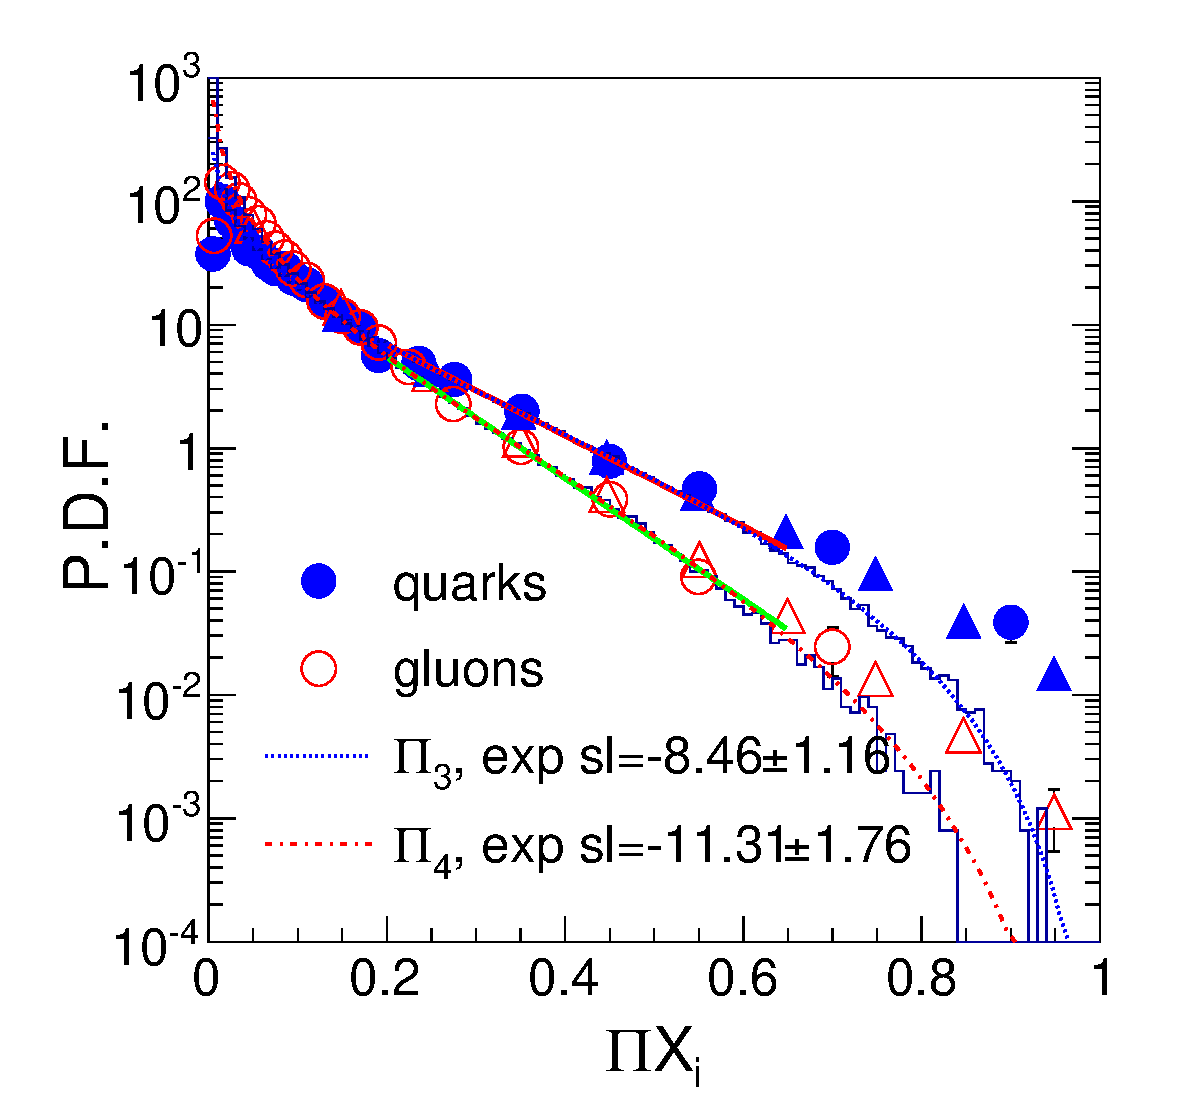
\includegraphics{figs/sumProd2}}
\resizebox{0.49\columnwidth}{!}{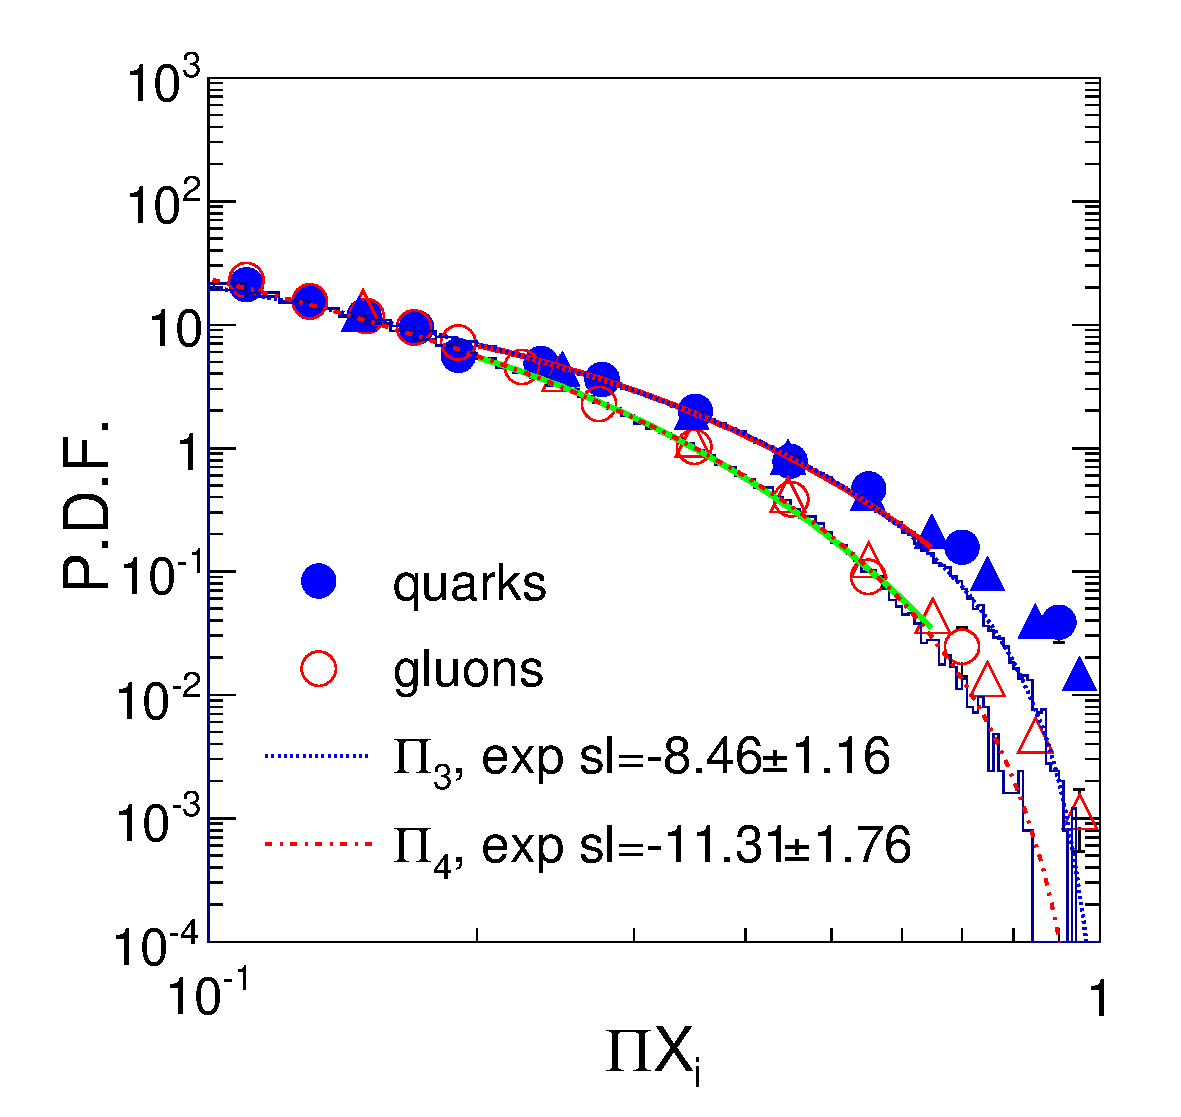
\includegraphics{figs/sumProd3}}
\caption{Product of 3 and 4 RVs compared to quark and gluon fragmentation functions. The product is is fitted in the middle region in order to extract the exponential slope as we did in \cite{Adler:2006sc}. Right plot is the same as left only in Log-x.}
\label{fig:sumProd}
\end{figure}

%------------------------------------------------------------------------------------------------------
\section{Jet cross section}

PCR \eq{eq:dsigma_integral} can be also used to evaluate the 
the ratio of the number of parons at a given transverse momentum to the number of charged particles at the
same \pt{}. From \eq{eq:dsigma_integral} it is easy to see 
\begin{equation}\label{eq:pcr}
R_{\rm PC}(\pt{}) \equiv \frac{d\sigma_{\rm parton}/d\pt{}}{d\sigma_{\rm h^\pm}/d\pt{}}\Biggl\vert_{h\pm} = \left(\int_{\xt}^{1} dz \cdot\D(z)\cdot z^{n-2}\right)^{-1}
\end{equation}

\begin{figure}[htbp]
   \centering
   \subfigure[]{ \label{fig:horowitz}   \resizebox{0.49\columnwidth}{!}{\includegraphics[viewport=0 -20 349 442,clip=]{horowitz}}  }
   \subfigure[]{ \label{fig:invar}   \resizebox{0.46\columnwidth}{!}{\includegraphics{papinvar}} }
   \caption{Left: The \pt{} dependencies of the power law exponent of partonic distributions for various c.m. energies from \cite{Horowitz:2011gd}. Right: Inclusive charged hadron \pt{} distribution for \s=0.9 TeV (red empty triangles) and \s=7 TeV (blue open diamonds) compared to NLO calculation \cite{Jager:2002xm}. Solid symbols represent the jet cross section calculated according \eq{eq:pcr} 
   (values in \tab{tab:pcr}).}  
\end{figure}

At LHC energy regime the \pt{} variation of \eq{eq:pcr} is much smaller than at lower energies due to the large phase space. This variation 
was negligible already at RHIC but it starts to be important at ISR. This makes the jet cross section estimation based on the PCR quite reliable at LHC. Another important condition for PCR is that the power law exponent $n$ characterizing the partonic cross section does not
vary with transverse momentum. Here, again due to the same phase space argument one can conclude that $n$ is more constant at LHC than at lower energies. Furthermore the NLO calculation supports this view as well \cite{Horowitz:2011gd} (see left panel of \fig{fig:horowitz}). Numerical integration of \eq{eq:pcr} for the fragmentation function from \tab{tab:FF} are summarized in \tab{tab:pcr}

\begin{table}[htdp]
\caption{Jet cross section /particle cross section ratio for three different fragmentation functions \tab{tab:FF} according \eq{eq:pcr}.}
\begin{center}
\begin{tabular}{l|c|c|c}
											& quark 	&  (quark+gluon)/2 	& gluon \\\hline
$R_{\rm PC}^{0.9 \rm TeV}$ 	($n=6.99\pm0.08$)		& 51.40  	& 100.00			& 184.94 \\
$R_{\rm PC}^{7 \rm TeV}$ 	($n=6.033\pm0.003$)	& 29.76  	& 50.71			& 81.75 \\
\end{tabular}
\end{center}
\label{tab:pcr}
\end{table}%
 
For both  \s=0.9 and 7 TeV cross sections we assumed purely  gluonic  $R^{\rm g}_{\rm PC}$ and the systematic errors were calculated as a difference between jet cross section calculated using $R^{\rm g}_{\rm PC}$ and $R^{\rm (q+g)/2}_{\rm PC}$. Resulting cross sections are shown on the left panel of \fig{fig:horowitz}.


\section{Comparison to NLO and PYTHIA}

Somewhat simplified approach is presented in \cite{Tannenbaum:2006ku}. When the fragmentation function is approximated by
a simple exponential function $D(z)=b^2\exp(-bz)$ then integral \eq{eq:pcr} has an analytical solution
\begin{equation}\label{eq:gamma}
R_{\rm PC}(\pt{})={\Gamma[n-1]\over b^{n-3}}\ .
\end{equation}
For a comparison, $R_{\rm CP}$ values for RHIC \piz{} distribution $\propto\pt{}^{-8.1}$ produced in \pp{} collisions are summarized in \tab{tab:RHIC}. It is evident that \eq{eq:gamma} from \cite{Tannenbaum:2006ku} is quite a good approximation of \eq{eq:pcr}.

\begin{table}[htdp]
\caption{Values of $R_{\rm CP}$ computed for RHIC c.m. energy \cite{Tannenbaum:2006ku} according  \eq{eq:gamma} and (\ref{eq:pcr}). }
\begin{center}
\begin{tabular}{l|l|r|r}
\fq{}=$\hat{C}\ptq{}^{-n}$.  & $\D=b^2\exp(-bz)$  	& \eq{eq:gamma} 	& \eq{eq:pcr} \\\hline
\multirow{2}{*}{$n$=8.1}    &  $b$=11.4 (gluon)  	&		282.7	&  303.3 \\
					  & $b$=8.2 (quark) 		&		52.7		& 75.5
\end{tabular}
\end{center}
\label{tab:RHIC}
\end{table}

\section{However}

In order to verify the method of extracting jet cross section a comparison to the PYTHIA, TOY simulation and NLO calculations \cite{Jager:2002xm} has been done.
In the case of PYTHIA the invariant $h^{\pm}$ distribution was studied together with the invariant spectrum of outgoing hard partons (status $\pm$23). Ratio of outgoing partons over the $h^{\pm}$ in $|\eta|<0.8$ at \s=7 TeV is shown on \fig{fig:jetcrosssection}. The NLO calculations for \s= 0.9 and 7 TeV are shown as well. It is evident that the PYTHIA $R_{\rm PC}$ overestimates the NLO calculation by a factor of 15 (scaled NLO by a factor of 15 showed by red dashed curve). On the other hand, the scaled NLO agrees with PYTHIA quite well.
$R_{\rm PC}$ value calculated according to \eq{eq:pcr} and represented by the solid horizontal line seem to approach NLO calculation at 
high \pt{}.

In conclusion, NLO prediction and calculation according \eq{eq:pcr} seem to agree at $\pt{}\gtrsim 30$ \gevc. However, PYTHIA shows values larger by factor of 15 ?! It the following section I will argue that the factor of 15 comes from an incorrect treatment of the fragmentation function. I cannot, however, explain why the NLO cross section ratio is so small.

\begin{figure}[htbp]
   \centering
   %\resizebox{0.49\columnwidth}{!}{\includegraphics[viewport=54 56 456 821,clip=]{}} 
   \resizebox{0.7\columnwidth}{!}{\includegraphics{qg}} 
   \caption{Ratio of outgoing parton over the $h^{\pm}$ cross section in $|\eta|<0.8$ at \s=7 TeV from PYTHIA (open circles). The NLO calculation for \s= 0.9 and 7 TeV are represented by solid and dashed curves (scaled NLO by factor of 15 showed by red dashed curve). 
$R_{\rm PC}$ value calculated according \eq{eq:pcr} is represented by a solid horizontal line. Horizontal dashed line represent  \eq{eq:pcr}
with the fragmentation function normalized to unity (see text below).
}  
   \label{fig:jetcrosssection}
\end{figure}

\section{Where is the factor of 15 coming from?}

I think, the reason is coming from the calculation of the joint probability formulae (\ref{eq:jointprob})-(\ref{eq:jointprobInv}) where both \fq{} (actually \ptq{}\fq) and $\D(z)$ are treated as probability distributions. It means that the normalization of the fragmentation function 
\eq{eq:pure_meanz} is inadequate and $\int_0^1\D(z)dz=1$ should be used instead.

In order to get more insight, a simple TOY simulation was used. First the RHIC case was studied: (i) The parton spectrum was simulated 
according the $\fq\propto\ptq{}^{1-n}$ where $n$=8.1 and \D{} according exponential function $\exp(-bz)$ where $b=8.2$ for a quark and $b=11.4$ for a gluon fragmentation functions \cite{Tannenbaum:2006ku}. Results are shown \fig{fig:toya}-\ref{fig:toyf}.

\fig{fig:toya} and \fig{fig:toyd} shows the comparison of the parent parton distribution fragmenting into a hadron of \pt{}=4 \gevc\ for quark
and gluon fragmentation function ($b=8.2$ and 11.4). Following \eq{eq:jointprobInv},  the parent parton distribution can be expressed as
\begin{equation} \label{eq:parent}
        {d^2\sigma_h\over d\ptq{}dz} = \hat{C}\left(\ptq{}\right)^{1-n}\cdot\D(z)
    %\makebox[5 mm]{}\rightarrow \makebox[5 mm]{}
    \rightarrow
            {d^2\sigma_h\over d\ptq{}d\pt{}} = \hat{C}\left(\ptq{}\right)^{-n}\cdot\D\left({\pt{}\over\ptq{}}\right)
\end{equation}
There is a clear agreement between \eq{eq:parent} and the toy simulations confirming the correctness of used formalism. Similar agreement can be observed in the case of the parent parton \mean{\zt} distribution from toy simulation compared to \eq{eq:meanz_inc}
(\fig{fig:toyb} and \ref{fig:toye}). Average values of \mzt{}  from the toy simulation and the formulae agrees quite well (see \tab{tab:toy}). Furthermore, an excellent agreement is seen also in the case of $R_{\rm PC}$ calculated according 
\eq{eq:pcr} and the toy simulation (\fig{fig:toyc}-\ref{fig:toyf}). {\bf However, in this case, used fragmentation functions were not normalized according \eq{eq:pure_meanz} but to unity ($\int_0^1\D(z)dz=1$)!}

\begin{figure}[htbp]
   \centering
   \subfigure[]{ \label{fig:toya}   \resizebox{0.31\columnwidth}{!}{\includegraphics{toyParent}} }
   \subfigure[]{ \label{fig:toyb}   \resizebox{0.31\columnwidth}{!}{\includegraphics{toyMeanZt}} }
   \subfigure[]{ \label{fig:toyc}   \resizebox{0.31\columnwidth}{!}{\includegraphics{toyRPC}} }
   \subfigure[]{ \label{fig:toyd}   \resizebox{0.31\columnwidth}{!}{\includegraphics{toyParentq}} }
   \subfigure[]{ \label{fig:toye}   \resizebox{0.31\columnwidth}{!}{\includegraphics{toyMeanZtq}} }
   \subfigure[]{ \label{fig:toyf}   \resizebox{0.31\columnwidth}{!}{\includegraphics{toyRPCq}} }
   \caption{Parent parton distribution fragmenting into a hadron of \pt{}=4 \gevc{} for $b=11.4$ (a) and $b=8.2$ (d). 
   Solid lines correspond to \eq{eq:parent}. Parent of \pt{}=4 \gevc{} parton \mean{\zt} distributions for $b=11.4$ (b) and $b=8.2$ (e). 
   Solid lines represent \eq{eq:meanz_inc}. The \mean{\zt} values from the  \eq{eq:meanz_inc} and from the toy simulation are indicating 
   in the legend.  $R_{\rm PC}$ distributions for $b=11.4$ (c) and $b=8.2$ (f). 
   }  
\end{figure}

\clearpage
\begin{table}[htdp]
\caption{Comparison of the average values of \za{} and $R_{\rm PC}$ from formulae and TOY monte carlo.}
\begin{center}
\begin{tabular}{c|c|c|c}
					&					& \mzt			& $R_{\rm PC}$ \\\hline
\multirow{2}{*}{$b$=8.2}	& TOY simulation 		& 0.696$\pm$0.01	& 626$\pm$5	\\
					& \eq{eq:meanz_inc}	& 0.696			& 618	\\\hline
\multirow{2}{*}{$b$=11.4}	& TOY simulation 		&  0.584$\pm$0.02	& 3434$\pm$65		\\
					& \eq{eq:pcr}			& 0.584			& 3457		\\\hline
\end{tabular}
\end{center}
\label{tab:toy}
\end{table}%


\section{Summary}

It is evident that \eq{eq:pcr} is the only equation here which is sensitive to the normalization of the fragmentation functions. When 
$\int_0^1\D(z)dz=1$ is used then the $R_{\rm PC}$ values are larger exactly by factor \mean{m_{\rm f}} (see \eq{eq:pure_meanz})
\begin{equation}
R_{\rm PC,\int_0^1\D(z)dz=1} = \mean{m_{\rm f}}R_{\rm PC,\int_0^1\D(z)dz=\mean{m_{\rm f}}}
\end{equation}
where for the exponential function 
\begin{eqnarray}
\D(z) &=& b^2\exp(-bz) \rightarrow \int_0^1\D(z)dz=\mean{m_{\rm f}}\approx b\label{eq:mf}\\
\D(z) &=& \frac{b}{1-e^{-b}}\exp(-bz)\rightarrow \int_0^1\D(z)dz=1
\end{eqnarray}
normalized according \eq{eq:mf} $\mean{m_{\rm f}}\approx b$ and the difference in $R_{\rm PC}$ is just equal to the slope $b$.


\section{Jet multiplicity and the difference between fragmentation function and $dN/dz$}

In pQCD terminology the fragmentation function is related to the probability that parton of momentum \ptq{} fragments into a particle 
of the momentum \pt{} but it cannot be directly treated as a probability distribution. A parton of fixed energy generates the first offspring 
particle which takes a $z_0$ fraction of parton energy. Parton of energy smaller by factor of $(1-z_0)$ continues to fragment by subsequent fragmentation. This process continues until the remaining parton energy is fully exhausted by factor $\Pi_{i=1}^{n}(1-z_i)$. Fragments of parton of momentum \ptq{}  have then the $z$-distribution 
\begin{equation}
\frac{dN}{dz}=\Pi_{i=1}^{n}(1-z_i)
\end{equation}¥ 

\begin{figure}[htbp]
   \centering
   \subfigure[]{ \label{fig:}   \resizebox{0.48\columnwidth}{!}{\includegraphics{frag_KKP1}} }
   \subfigure[]{ \label{fig:}   \resizebox{0.48\columnwidth}{!}{\includegraphics{frag_KKP2}} }
   \subfigure[]{ \label{fig:}   \resizebox{0.48\columnwidth}{!}{\includegraphics{frag_KKP3}} }
   \subfigure[]{ \label{fig:}   \resizebox{0.48\columnwidth}{!}{\includegraphics{frag_KKP_LP}} }
   \caption{Left:  Right: }  
\end{figure}

$
{dN_{\rm bg}\over d\xe{}} \propto Ê\int_{\ptt{}_{\rm, min}}^{\ptt{}_{\rm, max}} Ê\int_{\phi_{1}}^{\phi_{2}} 
\, \ptt{}^{-n}\,B_{\ptt{}}\left(-\xe{} { \ptt{} \over \cos\Delta\phi } \right)\, {\ptt{} \over \cos\Delta\phi }\, d\Delta\phi \,d\ptt{}\,.
$

 where $\phi_{1}=\arccos\left(\mathrm{Max}\left[-\xe{}\,\ptt{}/\pta{}_{\rm, min}\,;\,-1 \right]\right)$ and $\phi_{2}=\arccos(-\xe{})$.




%
%----------------------------------------------------------------------------------------------------------
\clearpage
\section{Fragmentation function and \xe}

Variable \xe{} is defined as
\begin{equation}
\xe{} = - { \vec{p}_{\rm Ta}\cdot \vec{p}_{\rm Tt}   \over \ptt{}^{2}} =-{\pta{} \over \ptt{}} \cos\Delta\phi 
\simeq \frac{\za\ptq{a}}{\zt\ptq{t}} \big|_{\dphi\rightarrow\pi}
\simeq \frac{\za}{\zt} \big|_{\dphi\rightarrow\pi\wedge\kt{}\rightarrow 0}
\simeq \za \big|_{\dphi\rightarrow\pi\wedge\kt{}\rightarrow 0\wedge\zt\rightarrow 1}
\label{eq:xE} 
\end{equation} 
For back-to-back pairs ($\dphi\rightarrow\pi$) \xe\ is equal to the ratio $\za\ptq{a}/\zt\ptq{t}$. For small values of \kt{} when $\ptq{a}\simeq\ptq{t}$, \xe\ variable reflects the ratio \za/\zt.  Since 1970s It has been believed that the \xe{} distribution associated to the high-\pt{} charged particle or \piz\ reflects directly the fragmentation function \cite{CCOR_xe}. Why this was generally adopted  is evident from 
the last term of \eq{eq:xE}. If f \zt\ is sufficiently close to unity then $\xe\simeq\za$ and thus the \xe{} distribution has the same shape as the fragmentation function. There are good reasons for these assumption known as a "trigger bias" \cite{Jacob:1978mj} 
and the "Bjorken Parent-Child Relationship"  (PCR) \cite{Bjorken:1973kd}. More details follows in section \ref{sec:parent-child}.

The simulation is done in following steps:
\begin{enumerate}
\item Generate the di-jet four-momenta $(\ptq, 0,\ptq{})$, $(\ptq, 0,-\ptq{})$ in c.m. system by sampling from a flat distribution ((E,$p_{||}, \vpt{})$ notation). 
\item Generate random net-pair momentum \pn{} according 2D Gaussian of the variance $\sigma_{\pn}=\sqrt{2\rms{\kt{}}}$.
\item Apply a Lorentz boost to the back-to-back parton pair according formula given below.
\item Generate random \zt{} according Leading Particle (LP) fragmentation function according \eq{eq:LPFF}
\item Generate random \za{} according KKP fragmentation function according \eq{eq:FF}
\item Generate random \jt{} component and add it to calculated particle \pt{t,a} = $z_{t,a}\ptq{t,a}+\jt{}\cdot\vec{e}_{\perp}$
\end{enumerate}

Toy simulations (see \ref{sec:intro} and \fig{fig:gamma}) clearly demonstrates the connection between fragmentation function and the \xe\ distribution when the trigger  particle is identical to trigger jet (\zt=1.0 as it is in the case of the direct-$\gamma$ and \kt{}=0 \gevc) . When the away side jet is emitted at the angle different from $\pi$ then the \xe\ distribution becomes steeper. 
\begin{figure}[htbp]
   \centering
   %\resizebox{0.49\columnwidth}{!}{\includegraphics[viewport=54 56 456 821,clip=]{}} 
   \subfigure[]{ \label{fig:gamma}   \resizebox{0.48\columnwidth}{!}{\includegraphics{xe_gamma_q}} }
   \subfigure[]{ \label{fig:gamma3pi4} \resizebox{0.48\columnwidth}{!}{\includegraphics{xe_gamma_3pi4}} }
   \caption{Left: \xe{} distributions from the toy simulations with KKP parameterization \eq{eq:FF} of the quark  fragmentation function and 
   \zt=1.0 as it is e.g. in the case of $\gamma$-hadron correlations. An effect of \kt{} smearing is mimicked by away-side emission 
    at an angle $\dphi = 3\pi/4$ w.r.t. trigger jet shown on the right panel.}  
\end{figure}
\begin{figure}[htbp]
   \centering
   %\resizebox{0.49\columnwidth}{!}{\includegraphics[viewport=54 56 456 821,clip=]{}} 
   \subfigure[]{ \label{fig:gamma_qg}   \resizebox{0.48\columnwidth}{!}{\includegraphics{xe_gamma_qg}} }
   \subfigure[]{ \label{fig:gamma_hh}   \resizebox{0.48\columnwidth}{!}{\includegraphics{xe_dihad_qg}} }
   \caption{Left: \xe{} distributions from the toy simulations with KKP parameterization \eq{eq:FF} of the quark and gluon fragmentation 
   function, \zt=1.0 and \kt{}=0 \gevc. Righ: the same \xe-distributions as on the left panel but the trigger is a fragment carrying $\zt<1$ 
   (leading particle fragmentation according \eq{eq:LPFF}).}  
\end{figure}
This demonstrated at 
\fig{fig:gamma3pi4} where an effect of \kt{} smearing is mimicked by away-side particle emission at angle $\dphi = 3\pi/4$ w.r.t. trigger jet.
One can observe an enhancement the low-\xe{} part and increases the high-\xe{} slope.
Figure \ref{fig:gamma_qg} shows the simulated \xe-distributions with KKP parameterization \eq{eq:FF} of the quark and gluon 
fragmentation  function and \zt=1.0. Obviously in the case of no \kt-smearing the \xe-distribution follow exactly the fragmentation function.
However, when the trigger particle is a fragmented hadron carrying $\zt<1$ (\fig{fig:gamma_hh}) then the \xe{} distributions becomes flatter and the sensitivity to the actual shape of the fragmentation function is, to the large extend, suppressed.


\begin{figure}[htbp]
   \centering
   %\resizebox{0.49\columnwidth}{!}{\includegraphics[viewport=54 56 456 821,clip=]{}} 
   \subfigure[]{ \label{fig:gamma34} \resizebox{0.48\columnwidth}{!}{\includegraphics{pap_invXeSlope}} }
   \caption{\xe{} distributions in the case the away-side jets is emitted at an angle $\dphi = 3\pi/4$ w.r.t. trigger jet and fixed \zt=1.0}  
\end{figure}


\clearpage
\section{Various}

Generally, a conditional probability of parton \ptq{} fragmenting into a particle \pt{} can be written
\begin{equation}\label{eq:child}
\frac{dP}{d\pt{}}\Biggl\vert_{\ptq{}} = D\left(\frac{\pt{}}{\ptq{}}\right)\frac{dz}{\pt{}} = D\left(\frac{\pt{}}{\ptq{}}\right)\frac{1}{\ptq{}}
\end{equation}
and thus \pt{} distribution has the same shape as the fragmentation function. 
Conditional probability of particle \pt{} being a fragment of parton \ptq{} can be written
\begin{equation}\label{eq:parent}
\frac{dP}{d\ptq{}}\Biggl\vert_{\pt{}} = 
       \frac{dP}{d\ptq{}} \frac{dP}{d\pt{}}\Biggl\vert_{\ptq{}} \frac{d\ptq{}}{d\pt{}}= 
       \ptq{}^{-n} D\left(\frac{\pt{}}{\ptq{}}\right)\frac{1}{\pt{}}\ .
\end{equation}
Two examples of the parton distributions fragmenting into a \pt{}=10 \gevc\ particle are shown on \fig{fig:paret-child}. Final state parton spectrum is simulated according the $\ptq{}^{-6}$ and the fragmentation function is a simple exponential function $D(z)=\exp(-6z)$ (left panel) or parameterization \eq{eq:LPFF} (right panel). Lines represent \eq{eq:parent}.
\begin{figure}[htbp]
   \centering
   %\resizebox{0.49\columnwidth}{!}{\includegraphics[viewport=54 56 456 821,clip=]{}} 
   \resizebox{0.49\columnwidth}{!}{\includegraphics{fig-p-c}} 
   \resizebox{0.49\columnwidth}{!}{\includegraphics{fig-p-c-LP}} 
   \caption{Distribution of parent partons fragmenting into a 10 \gevc\ hadron from the toy simulation and \eq{eq:parent} (dashed line).
   Distribution of inclusive partons according power law $dN/d\ptq{}\propto\ptq{}^{-6}$ and the fragmentation function $D(z)\approx\exp(-6z)$ 
   (left panel) or leading particle fragmentation function according \eq{eq:LPFF} (right panel).
   }  
   \label{fig:paret-child}
\end{figure}

\section{Fragmentation function and \kt{}}



%\bibliographystyle{h-physrev3}
\bibliographystyle{prsty}
%\bibliography{axe}
\bibliography{/Users/janrak/papers/bib-mypapers,/Users/janrak/papers/bib-PHENIX}

\end{document}  
